


\begin{lemma}
  The diagonals of a square bisect each other at the right angles
  \label{vec/2006/16}
% \begin{enumerate}
% %     \item  The angle made by two sides of a square is always 90\degree
%      \item  
%      \item  If $AB \perp BC$, 
%      \begin{align}
%       \brak{\vec{A}-\vec{B}}^\top\brak{\vec{B}-\vec{C}}=0
%      \end{align}
     
% \end{enumerate}
\end{lemma}
$\because$
\begin{align}
  \frac{\vec {A} + \vec {C}}{2}&=\frac{1}{2}\cbrak{\myvec {1\\2}+\myvec {3\\8}} \\ &= \myvec{2\\5} = \frac{\vec {B} + \vec {D}}{2},
  \end{align}
  and 
  
\begin{align}
  \brak{\vec{A}-\vec{C}}^\top\brak{\vec{B}-\vec{D}}&=\myvec {-2 & 6}\myvec {6\\-2}= 0,
  \\
  \implies  \brak{\vec{A}-\vec{B}}^\top\brak{\vec{B}-\vec{C}}&=0
\end{align}
from Lemma \ref{vec/2006/16}, the given points form a square.  This is verified in 
Fig. \ref{vec/2006/16/fig:Square ABCD}.
%
\begin{figure}[h!]
  \centering
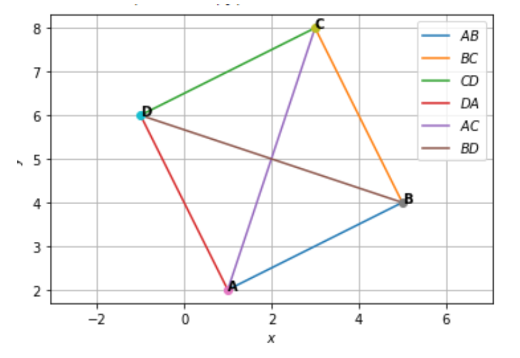
\includegraphics[width=\columnwidth]{vectors/solutions/2006/16/Python- Square Image.png}
  \caption{Square ABCD}
  \label{vec/2006/16/fig:Square ABCD}
\end{figure}


